% ===========================================================================
% ACT IV -- Reference Simulator  (Ch. 4)   Slides 28-40
% Budget: 7 minutes. Figure-dense; it moves fast if the images carry it.
% Every stage figure already exists and reproduces bit-for-bit from the
% notebook, so this is the best-supported act in the deck.
% ===========================================================================

\actdivider{4}{Reference Simulator}

% A stage slide. The stage figures are near-square three-panel stacks
% (1334x1181), so height is the binding dimension: putting the commentary in a
% side column lets the figure run nearly the full height of the frame.
% \stageslide{pip}{frame title}{image path}{commentary}
\newcommand{\stageslide}[4]{%
\begin{frame}{#2}
  \vspace{0.1em}
  \begin{columns}[T,onlytextwidth]
    \begin{column}{0.53\textwidth}
      \centering
      \includegraphics[width=\linewidth,height=0.80\textheight,keepaspectratio]{#3}
    \end{column}
    \begin{column}{0.44\textwidth}
      \raggedleft\stagepips{#1}

      \vspace{1.2em}
      \raggedright\small #4
    \end{column}
  \end{columns}
\end{frame}}

% --- 28. The validation argument -----------------------------------------
\begin{frame}{Built One Physical Effect at a Time}
  \vspace{0.2em}
  \begin{columns}[c,onlytextwidth]
    \begin{column}{0.46\textwidth}
      \centering
      \scalebox{0.70}{\stageLadder{0}}
    \end{column}
    \begin{column}{0.50\textwidth}
      \begin{itemize}\setlength\itemsep{0.6em}
        \item Each stage adds \textbf{one} physical effect and is tested on a
              case with a known expected result.
        \item All later results are \alert{measured against this simulator},
              so it must be correct.
        \item All nine stage figures can be regenerated from the notebook and
              match the originals \textbf{pixel for pixel}.
      \end{itemize}
    \end{column}
  \end{columns}
\end{frame}

% --- 29-37. The stages ----------------------------------------------------
\stageslide{1}{Stage 1: Single Powered Vehicle}%
  {../../notebooks/notebook_images/ltd_stage01_single_loco_traction_ramp_position_speed_netforce.png}%
  {Traction against rolling and air resistance (the Davis equation) on level
   track. Net force falls to zero as the vehicle reaches a steady speed. This
   confirms the integrator and the force signs before couplers are added.}

\stageslide{2}{Stage 2: Two Bodies, Linear Coupler}%
  {../../notebooks/notebook_images/ltd_stage02_loco_car_speeds_coupler_force_extension.png}%
  {The two speed traces overlap at this scale. \textbf{The coupler force and
   extension} show how the two vehicles interact.}

\begin{frame}{Stage 3: Nonlinear Coupler with Slack}
  \vspace{0.1em}
  \begin{columns}[T,onlytextwidth]
    \begin{column}{0.53\textwidth}
      \centering
      \includegraphics[width=\linewidth,height=0.80\textheight,keepaspectratio]%
        {../../notebooks/notebook_images/ltd_stage03_slack_coupler_linear_vs_nonlinear_force_delta_speeddiff.png}
    \end{column}
    \begin{column}{0.44\textwidth}
      \raggedleft\stagepips{3}

      \vspace{0.5em}
      \centering
      \scalebox{0.62}{\couplerLawChartPlain}

      \vspace{0.5em}
      \raggedright\small
      The coupler moves freely within $\pm 20$\,mm (the slack) before it
      transmits force, and is stiffer in one direction than the other. Shown
      against the Stage~2 linear coupler on the same run.
      \alert{The force now changes abruptly}, which is what slows the solver.
    \end{column}
  \end{columns}
\end{frame}

\stageslide{4}{Stage 4: Three Bodies and Force Propagation}%
  {../../notebooks/notebook_images/ltd_stage04_three_body_speeds_coupler_forces_train_stretch.png}%
  {Force travels down the chain one coupler at a time. End-to-end stretch is
   computed from the vehicle positions and previews how a long train behaves.}

\stageslide{4}{Stage 4b: Lead-Only Brake Pulse}%
  {../../notebooks/notebook_images/ltd_stage04b_lead_brake_pulse_speeds_coupler_forces.png}%
  {The run-in case: braking at the head end pushes the chain together. Compare
   the sign of the coupler forces against the previous slide.}

\stageslide{5}{Stage 5: General $N$-Vehicle Assembly}%
  {../../notebooks/notebook_images/ltd_stage05_N_vehicle_speeds_and_coupler_forces.png}%
  {The generalization from three bodies to arbitrary $N$, with no per-$N$
   special-casing anywhere in the force assembly.}

\begin{frame}{Stage 5: The Coupler-Force Heatmap}
  \vspace{0.1em}
  \centering
  \includegraphics[width=0.80\linewidth,height=0.62\textheight,keepaspectratio]%
    {../../notebooks/notebook_images/ltd_stage05_N_vehicle_coupler_force_heatmap.png}

  \vspace{0.3em}
  \begin{minipage}{0.88\textwidth}\small
    Force against time and coupler index. \textbf{Force decreases from front to
    rear} because the lead coupler pulls the entire trailing mass and the last
    coupler pulls a single car. The narrow band before $t \approx 20$\,s is the
    rising traction force travelling back through the slack.
  \end{minipage}
\end{frame}

\stageslide{6}{Stage 6: Per-Vehicle Grade and Curvature}%
  {../../notebooks/notebook_images/ltd_stage06_grade_profile_lead_rear_speeds_coupler_forces.png}%
  {Each vehicle reads the route at its own position. Lead and rear speeds
   differ wherever the train spans a change in grade, as described on
   slide~25.}

\stageslide{7}{Stage 7: Actuator Lag and Power-Limited Traction}%
  {../../notebooks/notebook_images/ltd_stage07_brake_buildup_power_limited_traction_states.png}%
  {First-order lag states for brake and traction, with tractive effort capped by
   available power at speed. A driving command changes these lag states, which
   then change the applied force.}

% --- 38. The brake-sign bug ----------------------------------------------
\begin{frame}{A Brake Sign Error and Its Fix}
  \vspace{0.1em}
  \begin{columns}[T,onlytextwidth]
    \begin{column}{0.49\textwidth}
      \centering
      {\footnotesize\color{uniCrimson}\textbf{As Published, Before 2026-08-17}}

      \vspace{0.2em}
      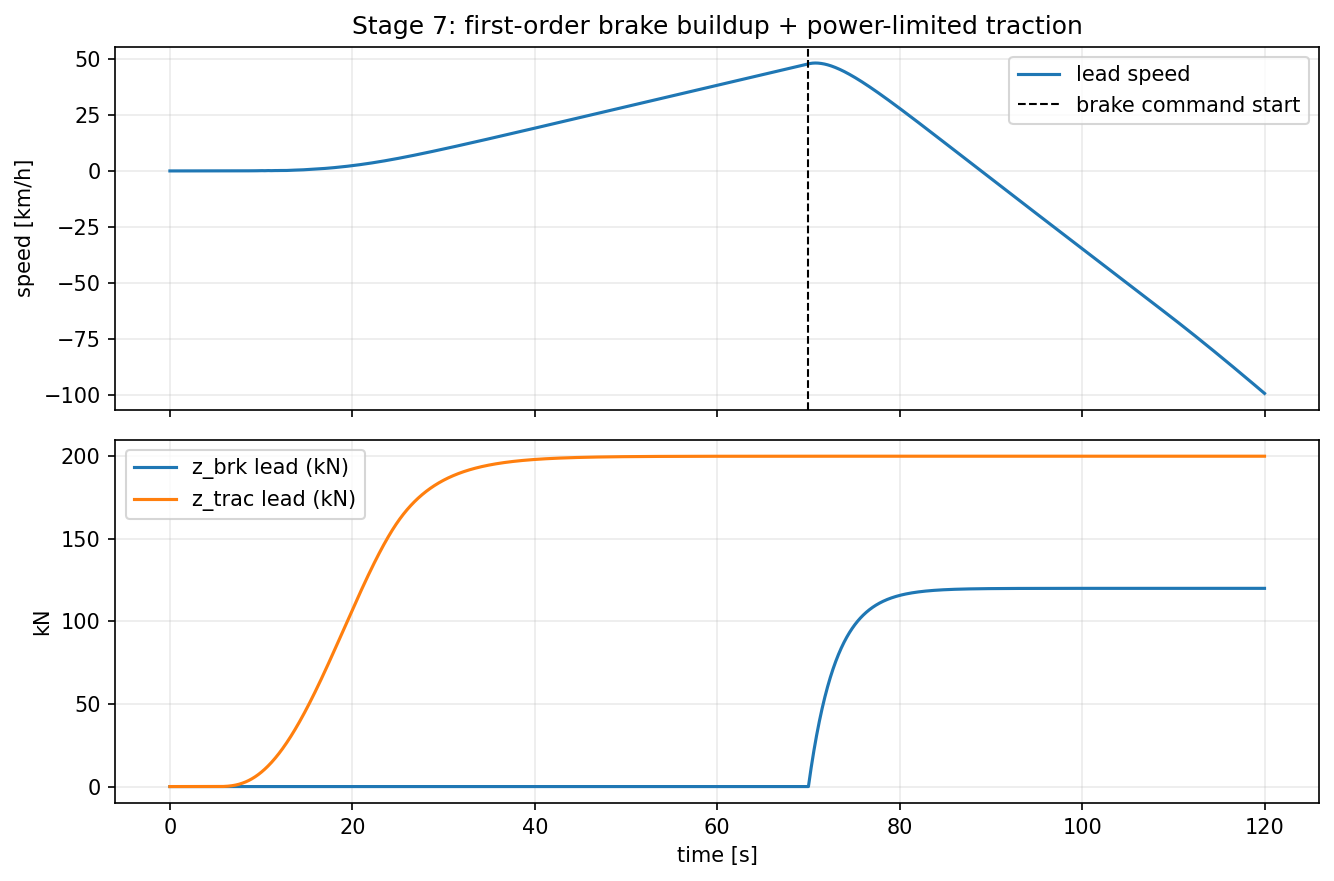
\includegraphics[width=\linewidth,height=0.52\textheight,keepaspectratio]{figures/ltd_stage07_prefix_brake_bug.png}
    \end{column}
    \begin{column}{0.49\textwidth}
      \onslide<2->{%
      \centering
      {\footnotesize\color{chartBlue!70!black}\textbf{Corrected}}

      \vspace{0.2em}
      \includegraphics[width=\linewidth,height=0.52\textheight,keepaspectratio]%
        {../../notebooks/notebook_images/ltd_stage07_brake_buildup_power_limited_traction_states.png}}
    \end{column}
  \end{columns}

  \vspace{0.3em}
  \begin{minipage}{0.96\textwidth}\footnotesize
    \only<1>{Brake force always pushed in the $-x$ direction, regardless of
      which way the train was moving. The speed passes through zero and keeps
      falling to \alert{$-99$\,km/h}: a train moving backward at 99\,km/h under
      full braking.}
    \only<2>{The fix makes brake force oppose the direction of motion, using a
      smooth $\tanh(v/\varepsilon)$ blend instead of $\mathrm{sgn}(v)$. The error
      went unnoticed because all earlier scenarios started from rest under
      traction. \textbf{Randomized starting conditions exposed it.} The fix
      changed \alert{only one} of the nine stage figures.}
  \end{minipage}
\end{frame}

% --- 39. Scope ------------------------------------------------------------
\begin{frame}{What the Simulator Is, and Is Not}
  \vspace{0.5em}
  \centering
  \scalebox{0.74}{\scopeTable}

  \vspace{1.0em}
  \begin{minipage}{0.92\textwidth}\small
    Parameters are \alert{realistic but not calibrated} to any specific
    locomotive or railcar. All results that follow measure agreement \emph{with
    this simulator}, not with real trains.
  \end{minipage}
\end{frame}

% --- 40. Tests ------------------------------------------------------------
\begin{frame}{Automated Tests}
  \vspace{0.6em}
  \begin{columns}[c,onlytextwidth]
    \begin{column}{0.34\textwidth}
      \centering
      \stattile{220}{Tests Passing}
      \vspace{0.5em}
      {\footnotesize 135 pre-existing \textbullet\ 60 torch acceptance\\
       10 dataset \textbullet\ 14 curvature}
    \end{column}
    \begin{column}{0.62\textwidth}
      \begin{itemize}\setlength\itemsep{0.6em}
        \item \texttt{test\_brake\_direction}: brakes never accelerate a
              stopped train, and brake force changes smoothly through zero
              speed. A hard $\mathrm{sgn}(v)$ fails the second check.
        \item \texttt{test\_tensorized\_matches\_classical}: the two
              implementations of the equations agree, with the brake option on
              and off.
        \item \texttt{test\_roeckl\_is\_discontinuous\_at\_300m}: confirms the
              jump in the \emph{published formula}, so the test fails if the
              formula is changed by mistake.
      \end{itemize}
    \end{column}
  \end{columns}
\end{frame}
